\section{Results}

For each episode, episode scores are calculated by summing up rewards of each time step. 
In \figref{fig:td3_scatter_ep_rewards} and \figref{fig:sac_scatter_ep_rewards}, a scatter plot is visualized for each model's episode scores. 
In \figref{fig:td3_std_ep_rewards} and \figref{fig:sac_std_ep_rewards}, moving average and standard deviation is visualized for each model's episode scores. 

\begin{figure}[!ht]
	\centering
	\begin{subfigure}{.49\textwidth}
		\centering
		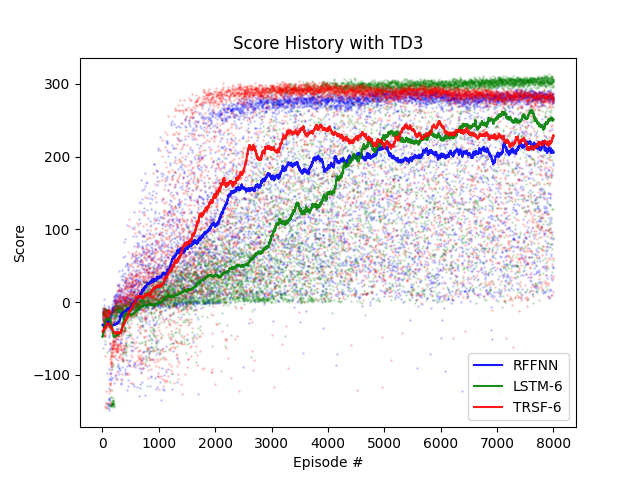
\includegraphics[width=0.99\textwidth]{figures/bipedal/SCT_TD3_RFFNN_LSTM-6_TRSF-6.png}
		\caption{TD3}
		\label{fig:td3_scatter_ep_rewards}
	\end{subfigure}
	\begin{subfigure}{.49\textwidth}
		\centering
		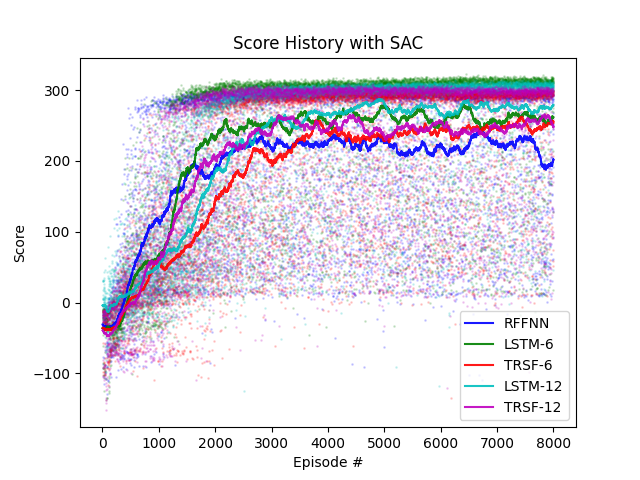
\includegraphics[width=0.95\textwidth]{figures/bipedal/SCT_SAC_RFFNN_LSTM-6_TRSF-6_LSTM-12_TRSF-12.png}
		\caption{SAC}
		\label{fig:sac_scatter_ep_rewards}
	\end{subfigure}
	\caption{Scatter Plot with Moving Average for Episode Scores (Window length: 200 episodes) for SAC}
\end{figure}

\begin{figure}[!ht]
	\centering
	\begin{subfigure}{.49\textwidth}
		\centering
		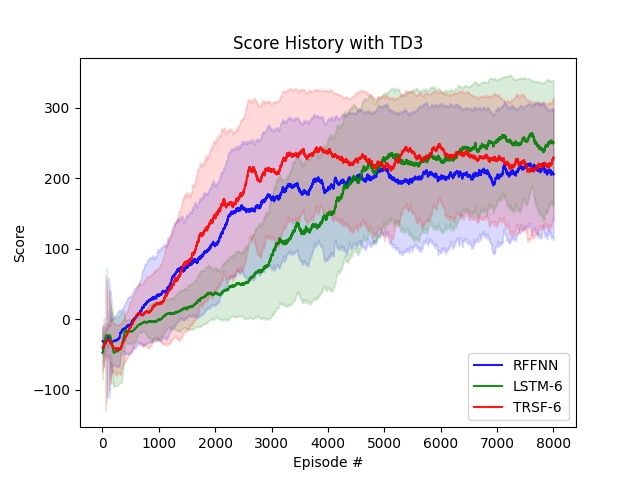
\includegraphics[width=0.99\textwidth]{figures/bipedal/STD_TD3_RFFNN_LSTM-6_TRSF-6.png}
		\caption{TD3}
		\label{fig:td3_std_ep_rewards}
	\end{subfigure}
	\begin{subfigure}{.49\textwidth}
		\centering
		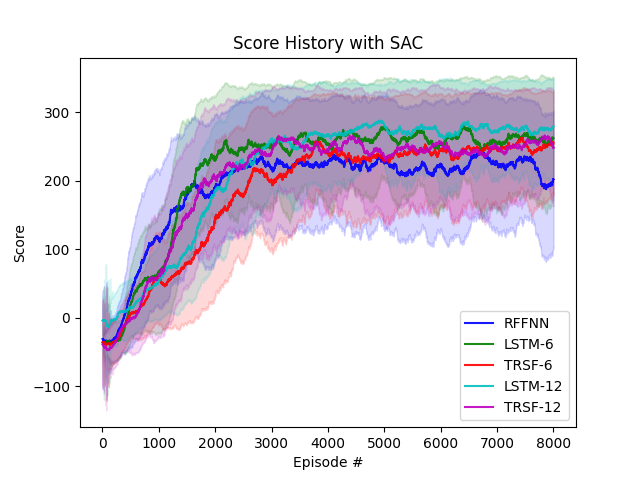
\includegraphics[width=0.95\textwidth]{figures/bipedal/STD_SAC_RFFNN_LSTM-6_TRSF-6_LSTM-12_TRSF-12.png}
		\caption{SAC}
		\label{fig:sac_std_ep_rewards}
	\end{subfigure}
	\caption{Moving Average and Standard Deviation for Episode Scores (Window length: 200 episodes) for TD3}
\end{figure}

RFFNN seems enough to make agent walk, although there exist partial observability in the environment. 
That model reaches around 221 points in average with TD3 and 245 points with SAC. 

Transformer models yield better performance compared to RFFNN. 249 points are reached by TD3 and 262 points reached by SAC model when 6 last observations are fed to model. 266 points are obtained when last 12 observations are fed to model with SAC.

LSTM model yield best results by reaching 264 points with TD3 and exceeds 280 points with SAC when 6 last observations are fed to model. 287 points are obtained when last 12 observations are fed to model with SAC. 

These scores are maximum obtained average scores of concurrent 200 episodes during training. 
However, while traning, model changes and agent still tries to explore envrionment. 
Officially, 300 points in average required in random 100 simulations to say the environment is solved~\cite{noauthor_gymleaderboard_2021}.
Therefore, best checkpoints are evaluated for 100 concurrent simulations without exploration. 
Results are summarized in \tabref{table:ckpt_performance}.

\begin{table}
\begin{center}
	\caption{Best checkpoint performances with 100 test simulations}
	\begin{tabular}{||c c c c||} 
		\hline
		RL Method & Model & Episode & Avg. Score \\ [0.5ex] 
		\hline\hline
		TD3 & RFFNN & 6600 & 207 \\ 
		\hline
		SAC & RFFNN & 7600 & 219 \\
		\hline
		TD3 & TRSF-6 & 6400 & 222 \\
		\hline
		SAC & TRSF-6 & 6800 & 254 \\
		\hline
		SAC & TRSF-12 & 6000 & 270 \\
		\hline
		TD3 & LSTM-6 & 7000 & 242 \\
		\hline
		SAC & LSTM-6 & 7600 & 268 \\
		\hline
		SAC & LSTM-12 & 7200 & 298 \\ [1ex] 
		\hline
	\end{tabular}
	\label{table:ckpt_performance}
\end{center}
\end{table}

None of our models exceed 300 point limit, but LSTM-12 model with SAC almost reaches to the limit \tabref{table:ckpt_performance}. 
However, all models partially solved problems by exceeding 200 point limit, while some simulations exceed 300 points with both TD3 (\figref{fig:td3_scatter_ep_rewards}) and SAC (\figref{fig:sac_scatter_ep_rewards}). 

Behaviour of agents are visualized in \figref{fig:rffnn_simulation}, \figref{fig:lstm_simulation} and \figref{fig:trsf_simulation} for SAC models. 
All of 3 models exhibit similar walking characteriscis.

SAC model performes better than TD3 in general, as seen in \figref{fig:td3_scatter_ep_rewards} and \figref{fig:sac_scatter_ep_rewards}. 
In addition, as seen from the moving average points, SAC agents are superior (\figref{fig:td3_std_ep_rewards},\figref{fig:sac_std_ep_rewards}).

\begin{figure}[!ht]
	\centering
	\begin{subfigure}{.95\textwidth}
		\centering
		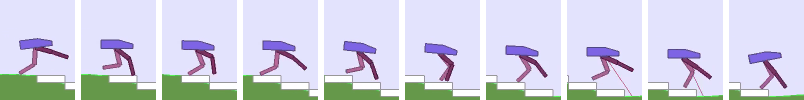
\includegraphics[width=0.95\textwidth]{figures/bipedal/anim/ff-stairs.png}
		\caption{Stairs}
		\label{fig:anim_rffnn_stairs}
	\end{subfigure}
	\begin{subfigure}{.95\textwidth}
		\centering
		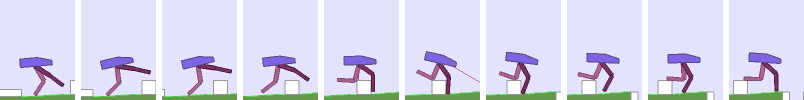
\includegraphics[width=0.95\textwidth]{figures/bipedal/anim/ff-hurdle.png}
		\caption{Hurdle}
		\label{fig:anim_rffnn_hurdle}
	\end{subfigure}
	\begin{subfigure}{.95\textwidth}
		\centering
		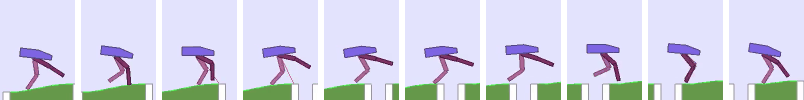
\includegraphics[width=0.95\textwidth]{figures/bipedal/anim/ff-pitfall.png}
		\caption{Pitfall}
		\label{fig:anim_rffnn_pitfall}
	\end{subfigure}
	\caption{Walking Simulation of RFFNN model at best version with SAC}
	\label{fig:rffnn_simulation}
\end{figure}

\begin{figure}[!ht]
	\centering
	\begin{subfigure}{.95\textwidth}
		\centering
		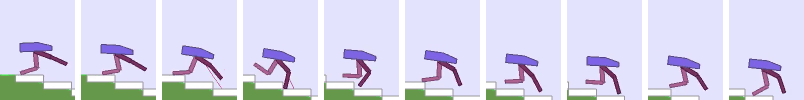
\includegraphics[width=0.95\textwidth]{figures/bipedal/anim/lstm-12-stairs.png}
		\caption{Stairs}
		\label{fig:anim_lstm_stairs}
	\end{subfigure}
	\begin{subfigure}{.95\textwidth}
		\centering
		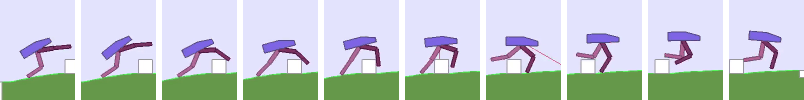
\includegraphics[width=0.95\textwidth]{figures/bipedal/anim/lstm-12-hurdle.png}
		\caption{Hurdle}
		\label{fig:anim_lstm_hurdle}
	\end{subfigure}
	\begin{subfigure}{.95\textwidth}
		\centering
		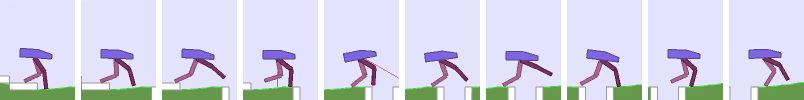
\includegraphics[width=0.95\textwidth]{figures/bipedal/anim/lstm-12-pitfall.png}
		\caption{Pitfall}
		\label{fig:anim_lstm_pitfall}
	\end{subfigure}
	\caption{Walking Simulation of LSTM-12 model at best version with SAC}
	\label{fig:lstm_simulation}
\end{figure}

\begin{figure}[!ht]
	\centering
	\begin{subfigure}{.95\textwidth}
		\centering
		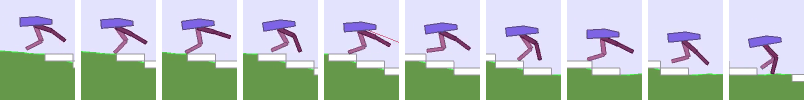
\includegraphics[width=0.95\textwidth]{figures/bipedal/anim/trsf-12-stairs.png}
		\caption{Stairs}
		\label{fig:anim_trsf_stairs}
	\end{subfigure}
	\begin{subfigure}{.95\textwidth}
		\centering
		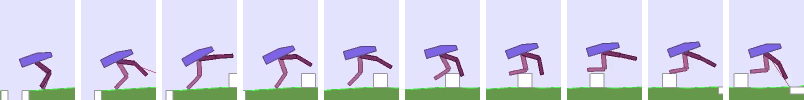
\includegraphics[width=0.95\textwidth]{figures/bipedal/anim/trsf-12-hurdle.png}
		\caption{Hurdle}
		\label{fig:anim_trsf_hurdle}
	\end{subfigure}
	\begin{subfigure}{.95\textwidth}
		\centering
		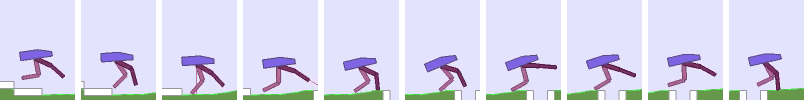
\includegraphics[width=0.95\textwidth]{figures/bipedal/anim/trsf-12-pitfall.png}
		\caption{Pitfall}
		\label{fig:anim_trsf_pitfall}
	\end{subfigure}
	\caption{Walking Simulation of Transformer-12 model at best version with SAC}
	\label{fig:trsf_simulation}
\end{figure}
